\begin{multicols}{2}
\begin{center}
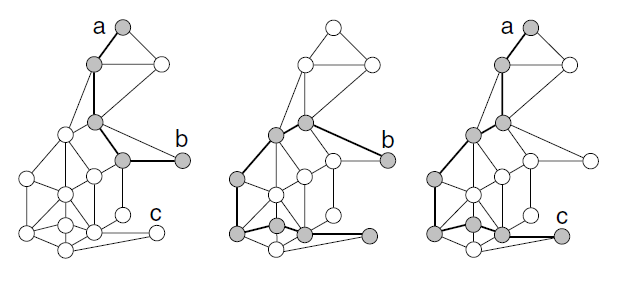
\includegraphics[width=75mm]{./graph_theory/path.png}
\end{center}
\subsection{Hechos y teoremas:}

\textbf{Camino euleriano:} Es un camino que pasa por todos los arcos exactamente una vez.\\
\textbf{Ciclo hamiltoniano:} Es un ciclo que contiene todos los nodos del grafo.\\
\textbf{Criterio de Euler:}
\begin{itemize}
\item Si un grafo conexo tiene mas de dos nodos con grado impar entonces no tiene un camino euleriano.
\item Si un grafo conexo tiene exactamente dos nodos con grado impar entonces tiene un camino euleriano. Todo camino euleriano debe comenzar en uno de esos nodos y terminar en el otro.
\item Si un grafo conexo no tiene nodos con grado impar entonces tiene un camino euleriano. Todo camino euleriano ser\'a cerrado.
\end{itemize}
Como consecuencia se tiene que un grafo tiene un camino euleriano cerrado si y solo si todos los nodos tienen grado par.\\
\textbf{Matriz laplaciana:} Para un grafo $G$ de $n$ vertices su matriz laplaciana $L:=(l_{i,j})_{n\times n}$ se define como:
\[
	l_{i,j}= \left\{ \begin{array}{ll}
		deg(v_i) &  \mbox{Si $i=j$}\\ 
		-1 & \mbox{Si $i\neq j$ y $v_i$ es adyacente a $v_j$}\\
		0 & \mbox{De lo contrario} \end{array} \right.
\]
\textbf{Teorema de Cayley:} El n\'umero de \'arboles \textit{etiquetados} de $n$ nodos es $n^{n-2}$.

\textbf{Teorema de Kirchhoff:} El n\'umero de \'arboles de expansi\'on de un grafo (etiquetado) es igual al valor absoluto de cualquier cofactor de la matriz laplaciana del grafo.
\end{multicols}
\subsection{Breadth-first Search}
{\small \emph{Breadth-First Search} (BFS) es una estrategia para recorrer todos los vertices de un grafo. M\'as especificamente el algoritmo BFS sirve para encontrar un vertice (o arco) que satisfaga una propiedad $P$ o para contar cuantos la satisfacen.
\pagebreak
	\algoritmo{./graph_theory/al-bfs}
\subsection{Depth-first Search}
	\algoritmo{./graph_theory/al-dfs}
\subsection{Algoritmo de Prim}
{\small Un \emph{spanning tree} o \emph{\'arbol de expansi\'on} de un grafo $G$ es un \'arbol $T$ que contiene todo vertice de $G$. Si un grafo tiene costos su \emph{minimum spanning tree} (MST) es un \'arbol de expansi\'on que tiene un peso total de arcos menor o igual al de cualquier otro posible \'arbol.}
	\algoritmo{./graph_theory/al-prim}
\subsection{Algoritmo de Dijkstra}
Para encontrar la distancia minima para ir desde un nodo $s$ a un nodo $d$. Dependiendo de que estructura se utilize para representar a $Q$ su complejidad varia. Por ejemplo si se hace con un heap
	\codigofuente{./graph_theory/dijkstra.java}
\subsection{Ordenamiento topol\'ogico:}
	\algoritmo{./graph_theory/al-topological-sort}
\subsection{Componentes fuertemente conexas:}
	\codigofuente{./graph_theory/ComputarSCC.java}
\pagebreak